\chapter{Proposed Methods}
\label{sq:methods}

To address the challenge in the question selection, 
we first introduce a learning-to-rank model 
with features found to be correlated with the question quality, in Section \ref{sq:ltr}. 
In addition, we propose a Transformer-based method for achieving a better ability to score questions in Section \ref{sq:dqs}.

\section{Learning-to-rank Question Selector}
\label{sq:ltr}
In the analysis of the developed dataset, we showed a large performance gap when the best and worst questions were asked.
Choosing the best question from a set of questions can be converted into a traditional Learning-To-Rank (LTR) problem. 
The goal of the model in LTR is to rank the elements in the given list. If the model can produce a ranking by scoring the questions in a given question set, 
it can be treated as a value function $V$ used to select the best question.
With the view of LTR, we proposed a method based on LambdaMART~\cite{burges2010ranknet}, which is a widely-used pairwise LTR model.


Based on the analysis of the dataset, we devised the following four features of each question $Q_t$, 
as the input of the proposed LTR model:
\begin{enumerate}
    \item The mean similarity of item pairs in the question $Q_t$.
    \item The similarity between the previous question $Q_{t-1}$ and the question $Q_t$.
    \item The category of fashion items in the previous question $Q_{t-1}$.
    \item The category of fashion items in the question $Q_t$.
\end{enumerate}
The similarity between two items is defined as the cosine similarity of their visual-semantic embeddings,
and the question similarity is defined in Equation \ref{eq:sim}.

\section{Deep Question Selector (DQS)}
\label{sq:dqs}

Although we included several features that can correlate to the quality of questions
in the LTR model,
the traditional approach using hand-crafted features may not fully 
capture the characteristics of questions. 
Hence, we propose a new deep neural network model for the question selection problem, to model the complex relationship between the previous questions and answers as well as question candidates. 

When designing the architecture of this new deep neural network model, 
there were two desiderata to effectively evaluate the quality of candidate questions:
\begin{enumerate}
    \item Questions should be modeled as a set of items, 
    and should not be treated as an average or a sequence of items.
    \item The past interaction or question-answering history should be modeled properly to avoid duplicate questions or not to receive less informative feedback. 
\end{enumerate}

\begin{figure}
  \centering
  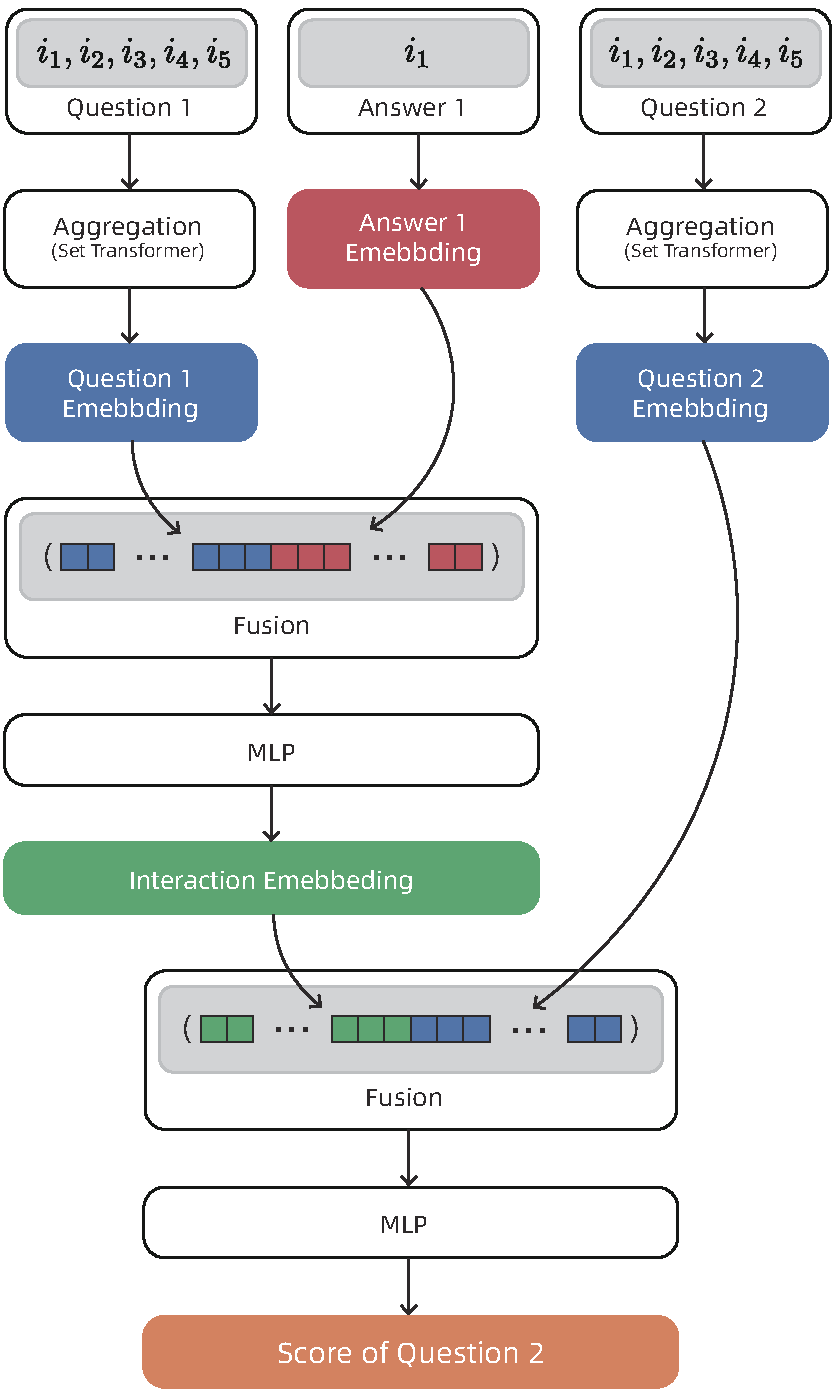
\includegraphics[width=0.6\linewidth]{figures/dqs.pdf}
  \caption{The architecture of Deep Question Selector (DQS).}
  \label{deep-model}
\end{figure}

Figure \ref{deep-model} illustrates the architecture of the proposed model
that can satisfy the two desiderata explained above. 
Questions are embedded by Set Transformer~\cite{lee2019set} in our model.
As we mentioned in the task setting, the question consists of $k$ items ($k=5$ in our case).
Although the input composed of multiple items is usually treated as a sequence in many machine learning scenarios, 
ours should be modeled by permutation-invariant models
since there is no order for items in a question.

Question-answer pairs are combined together and 
used as contextual information to estimate the value of candidate questions. 
A question-answering history $H_{t} = \{(Q_1, a_1), \ldots, (Q_t, a_t)\}$ can be embedded by iteratively applying a question-answering fusion and multilayer perceptrons:
\begin{eqnarray}
{\mathbf h}_t = g_t ([{\mathbf h}_{t-1}; [{\rm ST}_H(Q_{t}); {\mathbf a}_{t}]])
\end{eqnarray}
where ${\mathbf h}_t$ is the embedding for $H_t$,
${\rm ST}_H$ is Set Transformer for questions in the history,
and ${\mathbf a}_t$ is the embedding of the item given as an answer to the question $Q_t$.
The question-answer pair is combined by the vector concatenation operator $[;]$, and is further combined with the embedding of the question-answering history. 
A multilayer perceptron $g_t$ is repeatedly applied for keeping the embeddings in low dimensional spaces.
Figure \ref{deep-model} represents a special case of $t=1$ where only a question is asked and answered.
In this case, the question history ${\mathbf h}_1$ is obtained as follows:
\begin{eqnarray}
{\mathbf h}_1 = g_1 ([{\mathbf h}_{0}; [{\rm ST}_H(Q_{1}); {\mathbf a}_{1}]]) = g_1 ([{\rm ST}_H(Q_{1}); {\mathbf a}_{1}])
\end{eqnarray}
where ${\mathbf h}_0$ is defined as $\emptyset$
and $[\emptyset; x]$ is defined as $x$.

Given the question answering history $H_{t}$,
the value of a question conditioned by ${\mathbf h}_{t}$ is obtained by:
\begin{eqnarray}
V(H_{t}, Q) = g([{\mathbf h}_t; {\rm ST}(Q)])
\end{eqnarray}
where 
$g$ is a multilayer perceptron to produce a scalar value based on the embeddings of the question-answering history and question.
Note that Set Transformer, ${\rm ST}$, 
can be different from that used for embedding the past questions.
If Set Transformer ${\rm ST}_H$ shares parameters with the other Set Transformer ${\rm ST}$, 
the model is called \texttt{DQS-share}. 
Whereas if the parameters are not shared between two models, we call it \texttt{DQS-ind}.
These variants of the proposed model were compared in our experiments. 

The entire model contains two Set Transformer models ${\rm ST}_H$ and ${\rm ST}$,
multilayer perceptrons $g_t$ ($t=1, 2, \ldots$),
and a multilayer perceptron $g$ for outputting the question value.
They are trained with a cross entropy loss
of a classification problem where the task is to identify the best question among candidate questions.